\documentclass[letterpaper]{article}
\usepackage[utf8]{inputenc}
\usepackage[T1]{fontenc}
\usepackage[activeacute,spanish]{babel}
\usepackage[vmargin=4cm,tmargin=3cm,hmargin=2cm,letterpaper]{geometry}%
\usepackage{helvet}
\usepackage{amsmath,amsfonts,amssymb}
\usepackage{graphicx}
\usepackage{color}
\usepackage{xcolor}
\usepackage{verbatim}
\usepackage{tabls}
\usepackage{lastpage}
\usepackage{fancyhdr}
\usepackage{url}
\usepackage{listings}
%%%%%%%%%%%%%%%%%%%%%%%%%%%%%%%%%%%%%%%%%%%%%%%%%%%%%%%%%%%%%%%%%%%%%%%%%%%%%%%%%%%%%%%
\usepackage{tikz}
\usepackage{pgf}
\usepackage{pgffor}
\usepackage{pgfgantt}
\usepgfmodule{plot}
\usepackage{wrapfig}
\usetikzlibrary{arrows,decorations,snakes,backgrounds,fit,calc,through,scopes,positioning,automata,chains,er,fadings,calendar,matrix,mindmap,folding,patterns,petri,plothandlers,plotmarks,shadows,shapes,shapes.arrows,topaths,trees}

\lstset{% general command to set parameter(s)
%   basicstyle=\small,
  % print whole listing small
%   keywordstyle=\color{black}\bfseries\underbar,
  % underlined bold black keywords
%   identifierstyle=,
  % nothing happens
%   commentstyle=\color{white}, % white comments
%   stringstyle=\ttfamily,
  % typewriter type for strings
  showstringspaces=false}
  % no special string spaces

\pagestyle{fancy}
\color{black}
\fancyhead{}
\renewcommand{\headrule}{\hrule\vspace*{0.5mm}\rule{\linewidth}{0.8mm}}
\renewcommand{\familydefault}{\sfdefault}

\graphicspath{{./images/}}
\lhead{
\includegraphics[width=2cm]{logoucr.png}}
\rhead{
\includegraphics[width=3cm]{eie-text-gray-6x3cm.png}}
\chead{UNIVERSIDAD DE COSTA RICA\\FACULTAD DE INGENIERÍA\\ESCUELA DE INGENIERÍA ELÉCTRICA\\\textbf{ESTRUCTURAS ABSTRACTAS DE DATOS Y\\ ALGORITMOS PARA INGENIERÍA}\\IE-0217\\I CICLO 2014\\PROPUESTA DE PROYECTO DE ESTRUCTURAS DE DATOS Y ALGORIMTOS}

\lfoot{}%
\cfoot{}%
%\cfoot{\thepage\ de \pageref{LastPage}}%
\rfoot{}%

%%%%%%%%%%%%%%%%%%%%%%%%%%%%%%%%%%%%%%%%%%%%%%%%%%%%%%%%%%%%%%%%%%%%%%%%%%%%%%%%%%%%%%%%%%%%%%%%%%%%%%%%%%%%%%%
\newcommand{\uic}{black} %user-input color
%%%%%%%%%%%%%%%%%%%%%%%%%%%%%%%%%%%%%%%%%%%%%%%%%%%%%%%%%%%%%%%%%%%%%%%%%%%%%%%%%%%%%%%%%%%%%%%%%%%%%%%%%%%%%%%%%%
\newcommand{\uim}{} %user-input marker
%%%%%%%%%%%%%%%%%%%%%%%%%%%%%%%%%%%%%%%%%%%%%%%%%%%%%%%%%%%%%%%%%%%%%%%%%%%%%%%%%%%%%%%%%%%%%%%%%%%%%%%%%%%%%%%%%%
\newcommand{\userinput}[1]{\textcolor{\uic}{\uim#1\uim}}


%%%%%%%%%%%%%%%%%%%%%%%%%%%%%%%%%%%%%%%%%%%%%%%%%%%%%%%%%%%%%%%%%%%%%%%%%%%%%%%%%%%%%%%%%%%%%%%%%%%%%%%%%%%%%%%%%%
\begin{document}\vspace*{2cm}
%%%%%%%%%%%%%%%%%%%%%%%%%%%%%%%%%%%%%%%%%%%%%%%%%%%%%%%%%%%%%%%%%%%%%%%%%%%%%%%%%%%%%%%%%%%%%%%%%%%%%%%%%%%%%%%%%%

%%%%%%%%%%%%%%%%%%%%%%%%%%%%%%%%%%%%%%%%%%%%%%%%%%%%%%%%%%%%%%%%%%%%%%%%%%%%%%%%%%%%%%%%%%%%%%%%%%%%%%%%%%%%%%%%%%
\begin{center}
\Huge
\userinput{Análisis de complejidad y correctitud de los algoritmos de compresión y descompresión del sistema de empaquetado Ilsh(Implementación LZW-Hash)}
\vspace*{1cm}
\end{center}

\noindent
\small\baselineskip=14pt
\textbf{Estudiantes:} \\
\userinput{Willy Villalobos Marrero B17170}\\
\userinput{Daniel Méndez Zeledón A83911}\\
\userinput{Javier Acosta Villalobos A80056}\\

%%%%%%%%%%%%%%%%%%%%%%%%%%%%%%%%%%%%%%%%%%%%%%%%%%%%%%%%%%%%%%%%%%%%%%%%%%%%%%%%%%%%%%%%%%%%%%%%%%%%%%%%%%%%%%%%%%
\section{Introducción}

A partir de la segunda mitad del curso y como complemento de la programación en C++, se aprendió a realizar análisis que permiten determinar si los algoritmos son óptimos, que tan rápidos son y como mejorarlos. Como parte del proyecto, se va a tomar el algoritmo descrito por uno de los presentes en este proyecto como parte del curso y se le harán mejoras en caso de ser necesario, ademas de analizar su complejidad y su correctitud. El algoritmo que se va a analizar es el LZW utilizando tabla Hash, el cual genera un gran aporte a la compresión de los archivos.\\

\begin{figure}[h!]
	\centering
	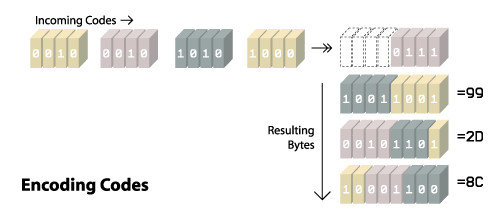
\includegraphics[width=0.5\textwidth]{lzw.jpg}
	\label{fig1}
	\caption{Muestra de compresión LZW}
\end{figure}

También, como parte del aporte al trabajo previo, se creará el algoritmo que descomprima los archivos de formato ilsh creados por el compresor y también se tratará de utilizar la teoría para hacer que éste sea lo más eficiente posible. De igual manera se le harán las respectivas pruebas de complejidad y correctitud paso por paso para así idenficar fallas del código como tal y las posibles mejoras a éstos.\\

\begin{figure}[h!]
	\centering
	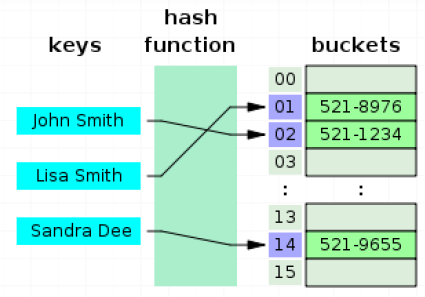
\includegraphics[width=0.3\textwidth]{Hash.png}
	\label{fig2}
	\caption{Tabla Hash}
\end{figure}

%%%%%%%%%%%%%%%%%%%%%%%%%%%%%%%%%%%%%%%%%%%%%%%%%%%%%%%%%%%%%%%%%%%%%%%%%%%%%%%%%%%%%%%%%%%%%%%%%%%%%%%%%%%%%%%%%%
\section{Objetivos}
\subsection{Objetivo General}

Analizar el algoritmo para la implementacion del LZW con tabla Hash con el fin de obtener su rendimiento a partir del análisis de correctitud y complejidad aprendidos en el curso para determinar si existe mejoras frente a otros compresores de archivos.

\subsection{Objetivos Específicos}

\begin{itemize}

\item Analizar la complejidad del algoritmo de compresión de LZW con tabla Hash para determinar el desempeño del algorimto, utilizando un análisis línea a línea de la cantidad de operaciones que hace éste.
\item Realizar un análisis de correctitud con el fin de demostrar que el algoritmo es correcto, utilizando los invariantes de lazo que se puedan determinar para tal demostración.
\item Crear el algoritmo para el descompresor que no se había tenido listo y a su vez analizar su complejidad y correctitud de la misma manera que para el compresor, de las formas previamente descritas.
\item Crear los esquemas del modelo de ejecución del algoritmo con el fin de tener una mejor representación del algoritmo y así mejorar su documentación.\\

\end{itemize}

%%%%%%%%%%%%%%%%%%%%%%%%%%%%%%%%%%%%%%%%%%%%%%%%%%%%%%%%%%%%%%%%%%%%%%%%%%%%%%%%%%%%%%%%%%%%%%%%%%%%%%%%%%%%%%%%%%
\section{Metodología}

Se hará un pequeño análisis previo, se verán las posibilidades de analizar eficazmente el algoritmo de compresión de LZW, una vez hecho esto, se hará un planeamiento de las tareas a realizar por cada uno de los miembros en conjunto, para acelerar el proceso de elaboración del documento final. Se comenzará por hacer el análisis de complejidad del algoritmo de compresión, a la vez que se va a crear el documento, por eso se le va a dar más tiempo para poder crear la tabla en formato \LaTeX  para su mejor presentación. A su vez, se comenzará a crear el algoritmo de descompresión que no se había hecho en la presentación de nuestro compañero, para finalizar con su análisis de complejidad. Una vez contruida la tabla y analizado el algoritmo, se trabajará conjuntamente para analizar ambos algoritmos respecto a su correctitud. Finalmente, se van a agregar los diagramas de flujos que no se habían hecho para la presentación de investigación pasada y se procederá a hacer una pequeña presentación para mostrar el proyecto a los presentes.

\begin{ganttchart}{0}{23}
	\gantttitle{Proyecto EDA}{24} \\
	\gantttitlelist{0,...,23}{1} \\
	\ganttgroup{PCL}{0}{23} \\
	\ganttbar{Análisis del algoritmo de compresión}{0}{2} \\
	\ganttbar{Planeamiento de tareas}{2}{3}
	\ganttnewline
	\ganttbar{Creación del documento final}{3}{20} \\
	\ganttbar{Análisis de complejidad Compresor}{3}{10}
	\ganttnewline
	\ganttbar{Creación del código de descompresión}{3}{10} \\
	\ganttbar{Análisis de complejidad Descompresor}{11}{15}
	\ganttnewline
	\ganttbar{Análisis correctitud compr. y descompr.}{15}{20} \\
	\ganttbar{Creación de la presentación}{20}{22}
	\ganttnewline
	\ganttmilestone{Previo a Exposición}{22}
	\ganttnewline
	\ganttbar{Expoisición PEDA}{23}{23}
	\ganttlink{elem1}{elem2}
	\ganttlink{elem2}{elem4}
	\ganttlink{elem2}{elem5}
	\ganttlink{elem4}{elem6}
	\ganttlink{elem5}{elem6}
	\ganttlink{elem6}{elem7}
	\ganttlink{elem7}{elem8}
	\ganttlink{elem8}{elem9}
	\ganttlink{elem9}{elem10}
	
\end{ganttchart}


%%%%%%%%%%%%%%%%%%%%%%%%%%%%%%%%%%%%%%%%%%%%%%%%%%%%%%%%%%%%%%%%%%%%%%%%%%%%%%%%%%%%%%%%%%%%%%%%%%%%%%%%%%%%%%%%%%
\section{Referencias}

\begin{enumerate}

\item Press, W., Teukolsky, W., Vetterling, W., Flannery, B. \textit{Numerical Recipes: The Art of Scietific Computing}, 3ra. Ed. Cambridge University Press, 2007
\item Cormen, T., Leiserson, C., Rivest, R., Stein, C. \textit{Introduction To Algorithms}, 3ra. Ed. MIT Press, 2009
\item Sedgewick, R., Wayne, K. \textit{Algorithms}, 4ta. Ed. Pearson Education, 2011
\item Eckel, B. \textit{Thinking in C++, volume I}, 2da. Ed. Prentice Hall, 2000
\item Referencias web: \begin{itemize}
	\item \url{http://oreilly.com/catalog/masteralgoc/chapter/ch08.pdf}
	\item \url{www.cs.princeton.edu/ rs/AlgsDS07/10Hashing.pdf}
	\item \url{http://burtleburtle.net/bob/hash/evahash.html}
	\item \url{http://cseweb.ucsd.edu/ mihir/cse207/w-hash.pdf}
	\item \url{http://www.sinfocol.org/herramientas/hashes.php}
	\end{itemize}

\end{enumerate}
	
\end{document}

